% Schematic representation of mach zender interferometer
% Modified from a version created by Henrik Kröger, https://github.com/derhedwig/fiberoptics/blob/master/auswertung.tex
% Author: Orlando Torres (2016)

\documentclass{standalone}
\usepackage{amsmath} % Required for \varPsi below
\usepackage{tikz,pgfplots}
\usetikzlibrary{calc}
\usetikzlibrary{patterns}
\usetikzlibrary{backgrounds}

\begin{document}
  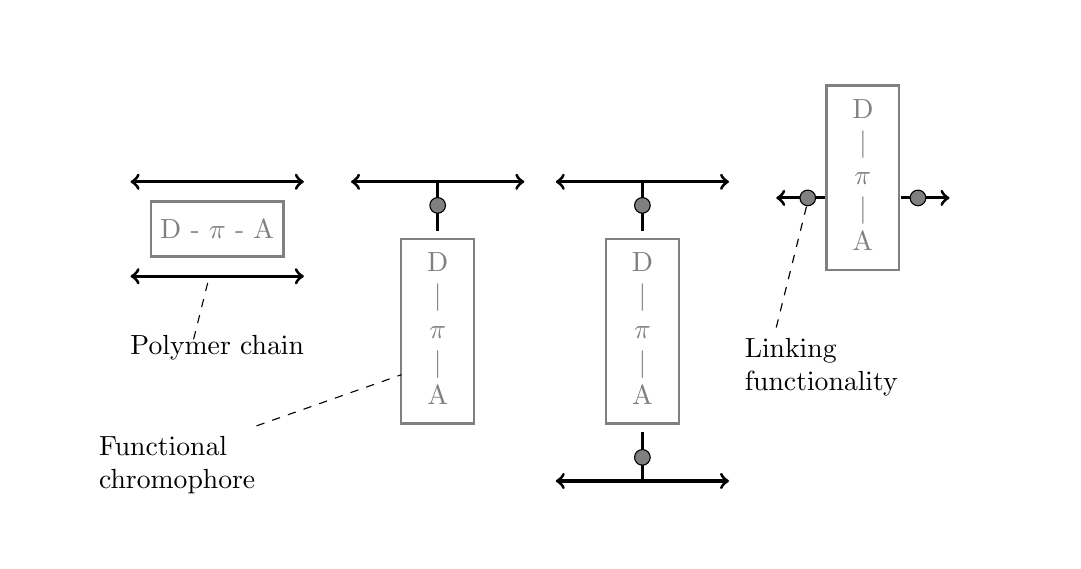
\begin{tikzpicture}
   	%define colors
    \definecolor{bbblue}{rgb}{0.262,0.709,0.613}
    \definecolor{rrred}{rgb}{0.933, 0.227, 0.286}
    \definecolor{yyyellow}{rgb}{0.933, 0.756, 0.227}
    
    %define coordinates for modulator (upper side)
    \coordinate (gh) at (-41.0mm, 0);
    \coordinate (sc) at (-13.0mm, -13mm);
    \coordinate (cl) at (13.0mm, -13mm);
    \coordinate (mc) at (41.0mm, 6.5mm);
    
    %\coordinate (ght) at (-67.0mm, 0);
    %\coordinate (ghe) at (-67.0mm, 0);
    %\coordinate (sc) at (-17.0mm, 0);
    %\coordinate (cl) at (17.0mm, 0);
    %\coordinate (mc) at (51.0mm, 0);
    
    % Functional chromophores %
    
    \node [shape=rectangle, minimum width=130mm, minimum height=65mm, draw=white]
    (bkgd) at (0,-7mm) {};
    
    \node [shape=rectangle,line width=0.3mm, minimum width=15mm, minimum height=7mm, color=gray, fill=white, draw]
    (guesthost) at (gh) {D - $\pi$ - A};
    \node [shape=rectangle,line width=0.3mm, minimum width=7mm, minimum height=15mm, color=gray, fill=white, draw]
    (sidechain) at (sc) {\begin{tabular}{c}D\\ $\lvert$ \\$\pi$ \\ $\lvert$ \\A\end{tabular}};
    \node [shape=rectangle,line width=0.3mm, minimum width=7mm, minimum height=15mm, color=gray, fill=white, draw]
    (crosslinked) at (cl) {\begin{tabular}{c}D\\ $\lvert$ \\ $\pi$  \\ $\lvert$ \\A\end{tabular}};
    \node [shape=rectangle,line width=0.3mm, minimum width=7mm, minimum height=15mm, color=gray, fill=white, draw]
    (mainchain) at (mc) {\begin{tabular}{c}D\\ $\lvert$ \\ $\pi$  \\ $\lvert$ \\A\end{tabular}};
	\begin{pgfonlayer}{background}
%    % Polymer chain %
 	%top polymer line guesthost
    \draw  [<->,line width=0.40mm, color=black] ($(guesthost)  + (11mm, +6mm)$) -- ($(guesthost) + (-11mm, +6mm)$);
    \draw  [<->,line width=0.40mm, color=black] ($(guesthost)  + (11mm, -6mm)$) -- ($(guesthost) + (-11mm, -6mm)$);
    
    % top sidechain
    \draw  [<->,line width=0.40mm, color=black] ($(sidechain)  + (11mm, +19mm)$) -- ($(sidechain) + (-11mm, +19mm)$);
    \draw  [-,line width=0.40mm, color=black] ($(sidechain)  + (0mm, 19mm)$) -- ($(sidechain) + (-0mm, 12.8mm)$);
    
    % top crosslinked
    \draw  [<->,line width=0.40mm, color=black] ($(crosslinked)  + (11mm, +19mm)$) -- ($(crosslinked) + (-11mm, 19mm)$);
    \draw  [-,line width=0.40mm, color=black] ($(crosslinked)  + (0mm, 19mm)$) -- ($(crosslinked) + (-0mm, 12.8mm)$);
    \draw  [<->,line width=0.40mm, color=black] ($(crosslinked)  + (11mm, -19mm)$) -- ($(crosslinked) + (-11mm, -19mm)$);
    \draw  [-,line width=0.40mm, color=black] ($(crosslinked)  + (0mm, -19mm)$) -- ($(crosslinked) + (-0mm, -12.8mm)$);
    %\draw  [<->,line width=0.40mm, color=black] ($(crosslinked)  + (11mm, -18mm)$) -- ($(crosslinked) + (-11mm, -18mm)$);
    
    % top mainchain
    \draw  [<-,line width=0.40mm, color=black] ($(mainchain)  + (-11mm, -2.55mm)$) -- ($(mainchain) + (-4.8mm, -2.55mm)$);
    \draw  [->,line width=0.40mm, color=black] ($(mainchain)  + (4.8mm, -2.55mm)$) -- ($(mainchain) + (11mm, -2.55mm)$);
    \end{pgfonlayer}
    %Linking functionalities
    \node [shape=circle, fill=gray, inner sep=2pt, draw]
    (scl) at ($(sidechain)  + (0mm, 16mm)$) {};
    \node [shape=circle, fill=gray, inner sep=2pt, draw]
    (cllt) at ($(crosslinked)  + (0mm, 16mm)$) {};
    \node [shape=circle, fill=gray, inner sep=2pt, draw]
    (clln) at ($(crosslinked)  + (0mm, -16mm)$) {};
    \node [shape=circle, fill=gray, inner sep=2pt, draw]
    (mcll) at ($(mainchain)  + (-7mm, -2.55mm)$) {};
     \node [shape=circle, fill=gray, inner sep=2pt, draw]
    (mclr) at ($(mainchain)  + (7mm, -2.55mm)$) {};
    
%    % Text %

\node [shape=rectangle,line width=0.0mm, minimum width=6mm, minimum height=10mm, draw=white]
    (pchain) at ($(guesthost)  + (0mm, -15mm)$) {Polymer chain};
\node [shape=rectangle,line width=0.0mm, minimum width=7mm, minimum height=10mm,  text width=22mm, draw=white]
    (lfunc) at ($(mainchain)  + (-4mm, -24mm)$) {Linking \\ functionality};
\node [shape=rectangle,line width=0.0mm, minimum width=7mm, minimum height=10mm, text width=30mm, draw=white]
    (fchrom) at ($(guesthost)  + (0mm, -30mm)$) {Functional \\ chromophore};

%    \draw (in) node [color=white] (in_node) at +(5mm, 0) { };
%    \draw (out) node [color=white] (out_node) at +(-5mm, 0)
%    { };
%    \node [align=center] (subs) at (38mm, -21mm) {Substrate}; 
%    \node (eleks) at (-28mm, -22mm) { };
%    \draw (in) node (sig_in) at +(5mm, 5mm) {Input};
%    \draw (out) node (sig_out) at +(-5mm, 5mm) {Output};
%    \draw (in1) node (wguideSt) [text width=10mm] at +(48mm, -22mm) {Strip \\ Waveguide};
%    \draw (in1) node (wguideSl) [text width=10mm] at +(-17mm, 12mm) {Slot \\ Waveguide};
%    \draw (phmod) node [text width=10mm] (generx) at +(-15mm, -22mm) {Phase \\ Modulator};
%    \draw (out2) node [text width=21mm] (StSlconv) at +(12mm, 28mm) {Strip-to-Slot \\ Converter};
%     \draw (out) node [text width=21mm] (mmi) at +(-5mm, -8mm) {MMI};
%    \draw (gen) node [text width=14mm] (pol) at +(-14mm, 23mm) {Poling \\Field};
%    \draw (gen) node [text width=14mm] (rf) at +(15mm, 23mm) {RF \\Field};
%        %\draw [dashed] (wguide) -- ($ (in0) + (3.3mm, 5mm) $);
%    %\draw [dashed] (eleks) -- (etop.west);
%    \draw [dashed] (wguideSt) -- ($(gen_node)  + (25mm, -3mm)$);
%    \draw [dashed] (mmi) -- ($(gen_node)  + (35mm, -3mm)$);
%    \draw [dashed] (StSlconv) -- ($(gen_node)  + (22mm, +9.34mm)$);
%    \draw [dashed] (wguideSl) -- ($(gen_node)  + (-16mm, +9.34mm)$);
    \draw [dashed] ($(pchain)  + (-3mm,1mm)$) -- ($(pchain)  + (-1mm, 9mm)$);
    \draw [dashed] ($(lfunc)  + (-7mm,5mm)$) -- ($(lfunc)  + (-3mm, 21mm)$);
    \draw [dashed] ($(fchrom)  + (5mm,5mm)$) -- ($(fchrom)  + (23.4mm, 11.5mm)$);
%     \draw [dashed] (pol) -- ($(gen_node)  + (-10mm, 12mm)$);
%      \draw [dashed] (rf) -- ($(gen_node)  + (8mm, 14.2mm)$);

  \end{tikzpicture}
%  \caption{Schematische Darstellung eines in Lithiumniobat (LiNbO$_3$) realisiertes
%  Mach-Zehnder-Modulators.}
%  \label{fig:mzm}
%\end{figure}
\end{document}